\documentclass[12pt]{article}
\usepackage[dvipsnames]{xcolor}
\usepackage[T1]{fontenc}
\usepackage{mathtools}
\usepackage[french]{babel}
\usepackage{amsmath,amssymb,amsthm}
\usepackage{array}
\usepackage{framed}
\usepackage{lmodern}
\usepackage{pdfpages}
\usepackage{listings}
\usepackage{adjustbox}
\usepackage{listingsutf8}
\usepackage{color}
\usepackage{tcolorbox}
\usepackage{algorithm}
\usepackage{algpseudocode}
\usepackage{graphicx}
\usepackage{subcaption}
\usepackage{hyperref}

\usepackage[a4paper,top=2cm,bottom=2cm,left=1.75cm,right=1.55cm,marginparwidth=1.75cm]{geometry}

\lstset{
  language=Java,
  basicstyle=\ttfamily\small, % Police de base en monospace
  keywordstyle=\color{blue}\bfseries, % Couleur des mots-clés
  stringstyle=\color{red}, % Couleur des chaînes de caractères
  commentstyle=\color{green!60!black}, % Couleur des commentaires
  numbers=left, % Numérotation des lignes à gauche
  numberstyle=\tiny, % Style de la numérotation
  stepnumber=1, % Numérote toutes les lignes
  frame=single, % Encadre le code
  breaklines=true, % Retour à la ligne automatique
  tabsize=4 % Taille des tabulations
}

% Useful packages
\usepackage{graphicx}
\usepackage[colorlinks=true, allcolors=blue]{hyperref}

% Configure the depth of the table of contents
\setcounter{tocdepth}{1}

\begin{document}

\includepdf{title.pdf}

\pagenumbering{arabic}
\hfill
\thispagestyle{empty}

\tableofcontents

\newpage

% INTRODUCTION
\section{Introduction}
\begin{quote}
    Dans un monde où les volumes de données augmentent de manière exponentielle, la gestion et le traitement efficace de ces données deviennent des enjeux majeurs. Le traitement d'images, en particulier, est un domaine clé dans de nombreuses applications, allant de l'imagerie médicale aux systèmes de reconnaissance visuelle. La complexité et la taille croissante des images nécessitent des solutions techniques capables de répondre aux exigences de rapidité, de scalabilité et de robustesse. \\

    Le projet \texttt{img-prc-mq} s'inscrit dans cette optique en proposant un système distribué de traitement d'images, en particulier de la compression, basé sur RabbitMQ, une solution de messagerie légère et performante. L'objectif est de concevoir et d'implémenter une architecture logicielle modulable, permettant d'uploader des images, de les compresser, puis de fournir les fichiers compressés aux utilisateurs finaux de manière efficace. \\

    Le choix de RabbitMQ s'explique par ses nombreux avantages, notamment la capacité à gérer des flux massifs de messages, sa flexibilité dans la mise en œuvre de modèles de communication asynchrones et son support natif pour la persistance des messages. Cette approche garantit un système évolutif et résilient, adapté à des charges de travail variables. \\

    L'architecture retenue repose sur des principes de découplage, de modularité et de scalabilité, en s'appuyant sur des microservices indépendants mais interconnectés. Chaque composant joue un rôle bien défini: Un serveur Flask gère les interactions avec les utilisateurs, des consumers RabbitMQ effectuent les tâches de traitement en arrière-plan, et RabbitMQ agit comme intermédiaire pour coordonner les flux de données entre les différents éléments. \\

    Ce rapport détaille les étapes clés de la conception et de l'implémentation de ce système, en mettant en avant les choix techniques, les défis rencontrés et les solutions adoptées pour atteindre les objectifs du projet.
\end{quote}

\newpage

% ARCHITECTUR LOGICIELLE
\section{Architecture logicielle}
\begin{quote}
    L'architecture logicielle de ce projet repose sur une communication asynchrone entre plusieurs composants clés : \\

    \begin{itemize}
        \item \textbf{Client} : User interface pour lancer les requêtes.
        \item \textbf{Serveur Flask} : Gère les interactions avec les utilisateurs (upload d'images, suivi de statut, téléchargement des fichiers compressés).
        \item \textbf{Consumers RabbitMQ} : Exécutent les tâches de traitement des images (compression).
        \item \textbf{RabbitMQ} : Agit comme un système de messagerie, orchestrant les interactions entre le serveur et les consumers. \\
    \end{itemize}

Cette architecture découplée permet une scalabilité et une résilience accrues, tout en assurant une maintenance simplifiée.

\begin{figure}[h!]
    \centering
    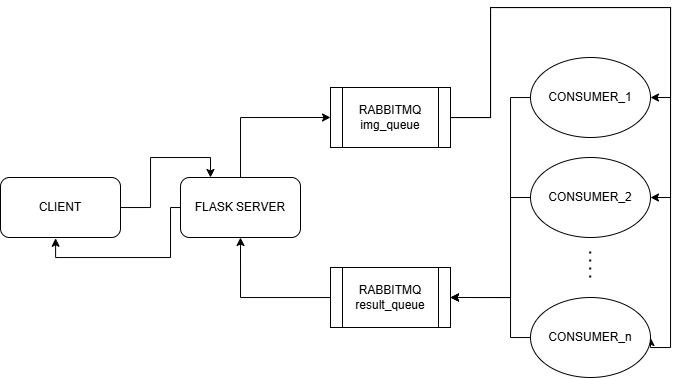
\includegraphics[width=0.8\textwidth]{architecture_diagram.png}
    \caption{Schéma de l'architecture logicielle}
    \label{fig:architecture}
\end{figure}


% FLASK SERVER
\subsection{Serveur Flask}
\begin{quote}
    
Le serveur Flask joue un rôle central dans l'architecture en tant que point d'entrée principal pour les utilisateurs et intermédiaire entre le client, RabbitMQ, et les consommateurs. Il est responsable des tâches suivantes : \\

\begin{itemize}
    \item \textbf{Upload des images} : 
    Le serveur reçoit les fichiers envoyés par les utilisateurs via une requête HTTP POST au point de terminaison \texttt{/upload}. Les images sont validées (type et extension), sauvegardées dans le dossier dédié \texttt{./uploads} (volume partagé), puis une tâche contenant le chemin du fichier et l'action à effectuer est publiée dans la file \texttt{TASK\_QUEUE} de RabbitMQ. \\
    
    Exemple de code pour l'upload et la publication d'une tâche dans RabbitMQ : \\
    
\begin{lstlisting}[language=Python]
@app.route('/upload', methods=['POST'])
def upload_image():
    if 'image' not in request.files:
        return jsonify({"message": "No file part"}), 400

    file = request.files['image']
    if file.filename == '':
        return jsonify({"message": "No selected file"}), 400

    if not allowed_file(file.filename):
        return jsonify({"message": "File type not allowed"}), 400

    file_path = save_file(file)
    task_message = json.dumps({"file_path": file_path, "action": "compress"})
    publish_message(RABBITMQ_SERVER, TASK_QUEUE, task_message)

    return jsonify({"message": "File uploaded successfully", "file_path": file_path}), 200
\end{lstlisting}
    \vspace{6mm}
    \item \textbf{Suivi du statut} : 
    Le point de terminaison \texttt{/status} permet aux utilisateurs de vérifier si leur image a été compressée. Si le traitement est terminé, un lien de téléchargement est généré dynamiquement. \\

    Exemple de code pour vérifier le statut d'une image compressée : \\
    
\begin{lstlisting}[language=Python]
@app.route('/status', methods=['GET'])
def check_status():
    file_name = request.args.get('file_name')
    if not file_name:
        return jsonify({"message": "File name is missing"}), 400

    compressed_path = os.path.join(app.config['DOWNLOAD_FOLDER'], f"compressed_{file_name}")
    if os.path.exists(compressed_path):
        download_url = url_for('download_file', file_name=f"compressed_{file_name}", _external=True)
        return jsonify({"status": "completed", "download_url": download_url}), 200
    else:
        return jsonify({"status": "processing"}), 200
\end{lstlisting}
\newpage
    \item \textbf{Téléchargement des images compressées} : 
    Une fois la compression terminée, les utilisateurs peuvent récupérer leur fichier via le point de terminaison \texttt{/download}. Le serveur sert les fichiers compressés à partir du dossier \texttt{downloads/} en tant que pièces jointes prêtes à être téléchargées. \\

    Exemple de code pour le téléchargement d'une image compressée : \\
\begin{lstlisting}[language=Python]
@app.route('/download', methods=['GET'])
def download_file():
    file_name = request.args.get('file_name')
    if not file_name:
        return jsonify({"message": "File name is missing"}), 400

    file_path = os.path.join(app.config['DOWNLOAD_FOLDER'], file_name)
    if not os.path.exists(file_path):
        return jsonify({"message": "File not found"}), 404

    return send_file(file_path, as_attachment=True)
    \end{lstlisting}
\end{itemize}

\subsubsection*{Principaux modules utilisés}
Le serveur utilise des libraries externes pour lancer le serveur, et la connexion à RabbitMQ \\

\begin{itemize}
    \item \textbf{Flask} : Framework léger pour gérer les requêtes HTTP et servir les fichiers.
    \item \textbf{Flask-CORS} : Gère les problèmes liés aux requêtes inter-origines (\textit{Cross-Origin Resource Sharing}).
    \item \textbf{pika} : Librairie Python pour interagir avec RabbitMQ.
    \item \textbf{Modules internes} :
    \begin{itemize}
        \item \texttt{utils.rabbitmq} : Pour publier et consommer des messages RabbitMQ.
        \item \texttt{utils.file\_handler} : Pour valider et sauvegarder les fichiers localement.
    \end{itemize}
\end{itemize}

\subsubsection*{Avantages}
\begin{itemize}
    \item \textbf{Modularité} : Une architecture découplée qui permet une maintenance simplifiée.
    \item \textbf{Simplicité d'utilisation} : Flask offre une interface intuitive pour gérer les requêtes utilisateur.
    \item \textbf{Scalabilité} : Facilité d'ajouter des fonctionnalités ou de supporter un plus grand nombre de requêtes.
\end{itemize}

\subsubsection*{Limites}
\begin{itemize}
    \item \textbf{Performance} : Sous une charge très importante, un équilibrage de charge (load balancing) serait nécessaire.
    \item \textbf{Résilience} : Une gestion centralisée des logs et des erreurs pourrait être ajoutée pour améliorer la robustesse.
\end{itemize}


\subsubsection*{Build}
Cette partie du projet peut se build (et lancer) via deux façons:
\begin{itemize}
    \item \textbf{Docker} : Dans le dossier \texttt{docker/} l'image \texttt{Docker.server} permet de lancer dans un conteneur pour mieux simuler un environement distribué.
    \item \textbf{Localhost} : Après certaines modifications expliquées dans le \href{https://github.com/napoknot21/img-proc-mq/blob/main/README.md}{README.md} du projet, on peut lancer localment le serveur.
\end{itemize}
\begin{figure}[h!]
    \centering
    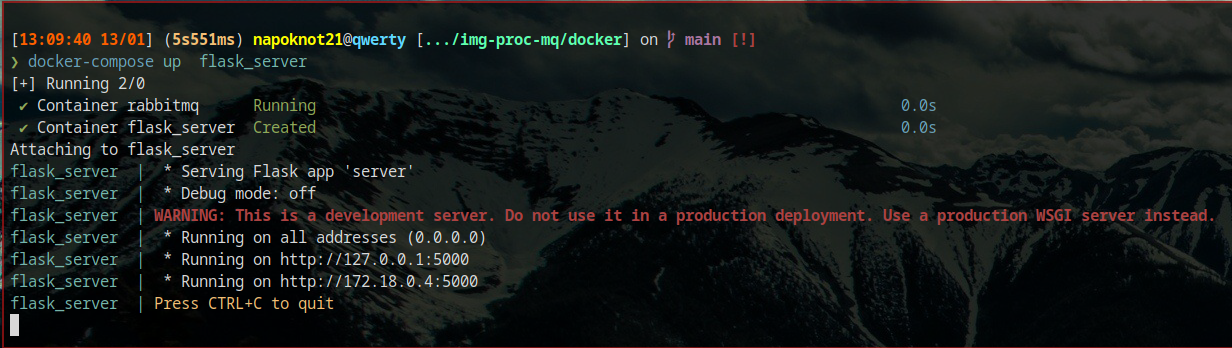
\includegraphics[width=0.8\textwidth]{flask_server.png}
    \caption{Lancement du serveur Flask}
    \label{fig:rabbitmq}
\end{figure}
\end{quote}

\subsection{Consumers RabbitMQ}
\begin{quote}

Les consumers RabbitMQ sont des composants essentiels de l'architecture. Ils exécutent les tâches de traitement des images (par exemple, la compression) qui leur sont assignées via RabbitMQ. Chaque consumer est indépendant, ce qui permet une scalabilité horizontale et une répartition efficace des charges. \\

\begin{itemize}
    \item \textbf{Réception des tâches} : Les consumers récupèrent les messages publiés dans la file \texttt{TASK\_QUEUE} par le serveur Flask.
    \item \textbf{Traitement des images} : Après avoir reçu une tâche, le consumer compresse l'image spécifiée en utilisant la bibliothèque \texttt{Pillow}.
    \item \textbf{Publication des résultats} : Les résultats (chemin de l'image compressée) sont publiés dans la file \texttt{RESULT\_QUEUE}, prêts à être consommés par le serveur Flask. \\
\end{itemize}

\subsubsection*{Fonctionnement général}
Le fonctionnement des consumers suit un workflow en trois étapes : \\
\begin{quote}
\begin{enumerate}
    \item Connexion à RabbitMQ et initialisation de la file \texttt{TASK\_QUEUE}.
    \item Consommation des messages contenant les informations sur les tâches.
    \item Compression des images et publication des résultats dans \texttt{RESULT\_QUEUE}.\\
\end{enumerate}
\end{quote}

Exemple de code pour la configuration et le démarrage d’un consumer : \\
\begin{lstlisting}[language=Python]
from rabbitmq.connection import get_channel
from core.compressor_consumer import process_message
from settings.config import RABBITMQ_SERVER, TASK_QUEUE

def main():
    connection, channel = get_channel(RABBITMQ_SERVER)
    channel.queue_declare(queue=TASK_QUEUE, durable=True)

    print(f"[*] Waiting for messages in {TASK_QUEUE}...")
    channel.basic_qos(prefetch_count=1)
    channel.basic_consume(queue=TASK_QUEUE, on_message_callback=process_message)

    try:
        channel.start_consuming()
    except KeyboardInterrupt:
        print("\n[-] Consumer stopped manually. Bye!")
    finally:
        connection.close()

if __name__ == "__main__":
    main()
\end{lstlisting}

\subsubsection*{Compression des images}
La compression est effectuée en utilisant la bibliothèque \texttt{Pillow}. \\
Chaque image est convertie en format \texttt{JPEG} avec une qualité spécifiée pour réduire sa taille. \\

Exemple de code pour la compression d’une image : \\
\begin{lstlisting}[language=Python]
import os
from PIL import Image

def compress_image (file_path) :
    try:
        with Image.open(file_path) as img:
            compressed_path = ROOT_STORAGE_FOLDER + DOWNLOAD_FOLDER + f"compressed_{os.path.basename(file_path)}"
            img = img.convert("RGB")
            img.save(compressed_path, "JPEG", optimize=True, quality=85)
            print(f"\n[+] Image compressed: {compressed_path}\n")
            return compressed_path
    except Exception as e:
        raise RuntimeError(f"[-] Failed to compress image: {e}")
\end{lstlisting}

\subsubsection*{Publication des résultats}
Une fois la compression terminée, les consumers publient les informations sur l'image compressée dans la file \texttt{RESULT\_QUEUE}, permettant au serveur Flask de finaliser le workflow. \\

Exemple de code pour la publication des résultats : \\
\begin{lstlisting}[language=Python]
from rabbitmq.publisher import publish_message
from settings.config import RESULT_QUEUE

def process_message(ch, method, properties, body):
    message = json.loads(body)
    file_path = message.get("file_path")

    try:
        compressed_path = compress_image(file_path)
        result_message = {"original_path": file_path, "compressed_path": compressed_path}
        publish_message(RESULT_QUEUE, result_message)
        ch.basic_ack(delivery_tag=method.delivery_tag)
    except Exception as e:
        ch.basic_nack(delivery_tag=method.delivery_tag)
\end{lstlisting}

\subsubsection*{Principaux modules utilisés}
\begin{itemize}
    \item \textbf{Pillow} : Pour effectuer les opérations de traitement et compression d'images.
    \item \textbf{pika} : Pour interagir avec RabbitMQ (consommation et publication des messages).
    \item \textbf{Modules internes} :
    \begin{itemize}
        \item \texttt{core.compressor\_consumer} : Pour le traitement des messages et la compression des images.
        \item \texttt{rabbitmq.connection} : Pour établir une connexion avec RabbitMQ.
        \item \texttt{rabbitmq.publisher} : Pour publier les résultats dans la file \texttt{RESULT\_QUEUE}.
    \end{itemize}
\end{itemize}

\subsubsection*{Avantages}
\begin{itemize}
    \item \textbf{Scalabilité horizontale} : Possibilité d'ajouter plusieurs instances de consumers pour traiter un grand volume de messages.
    \item \textbf{Indépendance} : Les consumers fonctionnent indépendamment du serveur Flask, permettant une meilleure modularité.
    \item \textbf{Résilience} : RabbitMQ garantit que les messages non traités restent disponibles jusqu'à leur consommation.
\end{itemize}

\subsubsection*{Limites}
\begin{itemize}
    \item \textbf{Performance limitée par le traitement} : Les tâches complexes comme la compression d'images volumineuses peuvent ralentir les performances.
    \item \textbf{Dépendance à RabbitMQ} : Si RabbitMQ devient indisponible, le traitement des tâches est interrompu.
\end{itemize}

\subsubsection*{Build}
Les consumers peuvent être exécutés dans différents environnements :
\begin{itemize}
    \item \textbf{Docker} : L'image Docker dédiée (\texttt{Dockerfile.consumer}) facilite le déploiement et l'exécution dans des conteneurs isolés.
    \item \textbf{Localhost} : En configurant les dépendances localement, il est possible de démarrer les consumers en local pour des tests rapides.
\end{itemize}
\begin{figure}[h!]
    \centering
    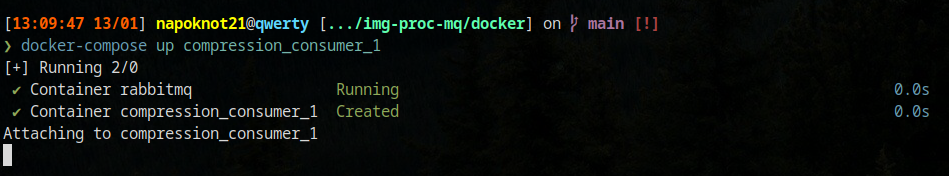
\includegraphics[width=0.8\textwidth]{compression_consumer.png}
    \caption{Lancement du consumer}
    \label{fig:rabbitmq}
\end{figure}
\end{quote}


\end{quote}

% RABBITMQ
\section{RabbitMQ}
\begin{quote}
RabbitMQ est au cœur de l'architecture logicielle, agissant comme un système de messagerie fiable et performant. Il facilite la communication asynchrone entre les différents composants, assurant le découplage et la scalabilité de l'ensemble du système.

\subsubsection*{Rôles principaux}
\begin{itemize}
    \item \textbf{Médiateur de messages} : RabbitMQ reçoit, stocke et distribue les messages entre le serveur Flask et les consumers.
    \item \textbf{Persistant et fiable} : Les messages dans les queues sont marqués comme durables, garantissant qu'ils ne sont pas perdus en cas de panne.
    \item \textbf{Orchestration des tâches} : Permet de gérer plusieurs instances de consumers en répartissant les messages selon le principe du round-robin.
\end{itemize}

\subsubsection*{Files utilisées et exemples de messages}
\begin{itemize}
    \item \textbf{TASK\_QUEUE} : \\
    Contient les messages envoyés par le serveur Flask pour les tâches à traiter. Chaque message inclut les informations suivantes :
    \begin{itemize}
        \item \texttt{file\_path} : Le chemin de l'image à traiter.
        \item \texttt{action} : L'action à effectuer (par exemple, \texttt{compress}).\\

        \textbf{Exemple de message envoyé par le serveur Flask :} 
        \begin{lstlisting}[language=json]
{
    "file_path": "./uploads/user_image.jpg",
    "action": "compress"
}
        \end{lstlisting}
    \end{itemize}
    \vspace{6mm}
    \item \textbf{RESULT\_QUEUE} : \\
    Contient les résultats générés par les consumers. Chaque message inclut :
    \begin{itemize}
        \item \texttt{original\_path} : Le chemin de l'image originale.
        \item \texttt{compressed\_path} : Le chemin du fichier compressé. \\

        \textbf{Exemple de message envoyé par un consumer :} 
        \begin{lstlisting}[language=json]
{
    "original_path": "./uploads/user_image.jpg",
    "compressed_path": "./downloads/compressed_user_image.jpg"
}
        \end{lstlisting}
    \end{itemize}
\end{itemize}

\begin{figure}[h!]
    \centering
    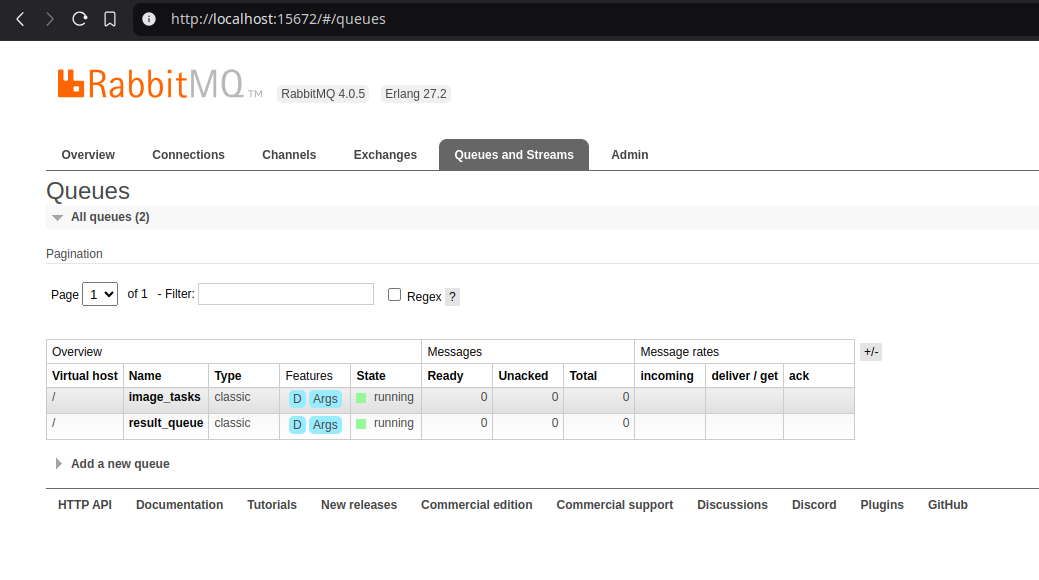
\includegraphics[width=0.8\textwidth]{queues.png}
    \caption{Queues créées sur RabbitMQ}
    \label{fig:rabbitmq}
\end{figure}


\subsubsection*{Configuration}
RabbitMQ est configuré pour assurer une communication fiable et performante :
\begin{itemize}
    \item Les queues (\texttt{TASK\_QUEUE} et \texttt{RESULT\_QUEUE}) sont déclarées comme \textbf{durables}, assurant la persistance des messages.
    \item Les \textbf{préférences de qualité de service} (QoS) sont configurées avec \texttt{prefetch\_count=1}, permettant à chaque consumer de traiter un message à la fois pour éviter les surcharges.
    \item L'authentification par défaut (\texttt{guest:guest}) est utilisée dans un environnement de développement, mais elle peut être personnalisée pour une utilisation en production.
\end{itemize}

\subsubsection*{Avantages de RabbitMQ}
\begin{itemize}
    \item \textbf{Découplage des composants} : Les services client, serveur et consumer fonctionnent indépendamment, ce qui simplifie leur maintenance et leur évolution.
    \item \textbf{Fiabilité} : Les messages non traités restent disponibles jusqu'à leur consommation, garantissant qu'aucune tâche n'est perdue.
    \item \textbf{Scalabilité horizontale} : RabbitMQ permet d'ajouter ou de retirer dynamiquement des consumers selon la charge du système.
\end{itemize}

\subsubsection*{Limites}
\begin{itemize}
    \item \textbf{Dépendance réseau} : En cas de défaillance de la connexion réseau entre le serveur Flask et RabbitMQ, les messages ne peuvent pas être publiés ou consommés.
    \item \textbf{Complexité en production} : Une configuration avancée est nécessaire pour garantir la sécurité, l'équilibrage de charge et la gestion des échecs.
\end{itemize}

%\subsubsection*{Schéma simplifié de RabbitMQ}
%\begin{figure}[h!]
%    \centering
%    \includegraphics[width=0.8\textwidth]{rabbitmq_diagram.png}
%    \caption{Schéma simplifié de la gestion des messages par RabbitMQ}
%    \label{fig:rabbitmq}
%\end{figure}

\subsubsection*{Build}
Dans le projet, RabbitMQ est lancé en tant que conteneur Docker via le fichier \texttt{docker-compose.yml}. Voici les principales configurations : \\
\begin{itemize}
    \item \textbf{Port 5672} : Utilisé pour les protocoles AMQP (Advanced Message Queuing Protocol).
    \item \textbf{Port 15672} : Utilisé pour l'interface de gestion Web.
    \item \textbf{Exemple de commande pour accéder à RabbitMQ via Docker :}
\begin{lstlisting}[language=bash]
docker-compose up rabbitmq
\end{lstlisting}
\end{itemize}

\begin{figure}[h!]
    \centering
    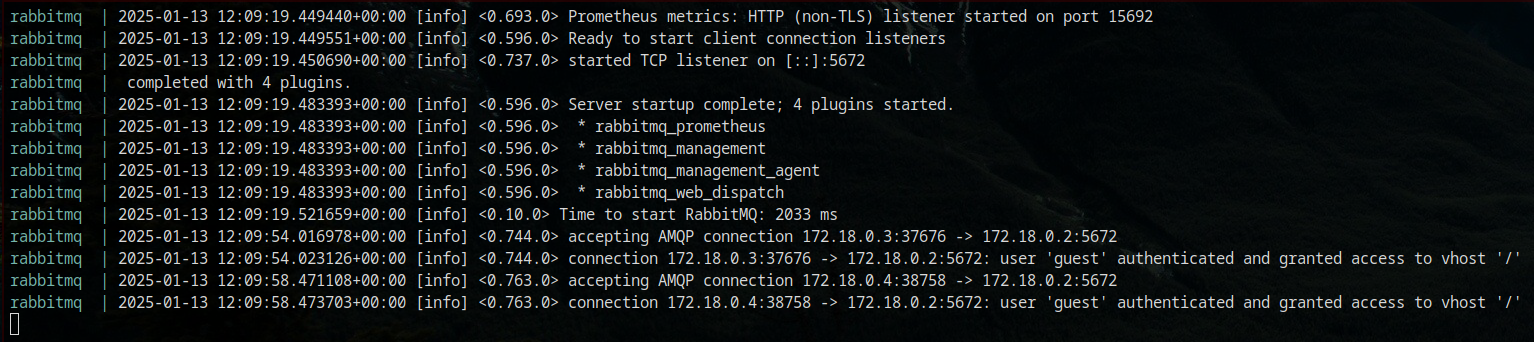
\includegraphics[width=0.8\textwidth]{rabbit_mq.png}
    \caption{Lancement de RabbitMQ sur Docker}
    \label{fig:rabbitmq}
\end{figure}

\end{quote}

\newpage


% CONCLUSION
\section{Conclusion et performances}
\begin{quote}
    
Ce projet a mis en œuvre une architecture logicielle basée sur RabbitMQ pour orchestrer un système distribué de traitement d'images. Le découplage des responsabilités entre les différents composants (serveur Flask, consumers RabbitMQ et client) a permis de créer une solution robuste et évolutive. La modularité de cette approche simplifie la maintenance et offre la possibilité d'étendre facilement les fonctionnalités.

\subsection{Performances du système}
L'architecture a démontré une réactivité satisfaisante dans les cas de test. Voici les principaux résultats observés : \\

\begin{itemize}
    \item \textbf{Temps de traitement moyen} : Une image de 3 MB est compressée en environ 2 secondes, incluant le temps de transfert des messages dans RabbitMQ.
    \item \textbf{Réduction de taille des images} : En moyenne, les images compressées atteignent 40\% de leur taille initiale, tout en conservant une qualité visuelle acceptable grâce à des réglages optimaux (qualité à 85\%).
    \item \textbf{Gestion de charge} : Avec l'ajout de plusieurs consumers, le système distribue efficacement les tâches, réduisant ainsi le temps d'attente global en cas de forte affluence.
    \item \textbf{Résilience} : Les tâches sont correctement conservées dans RabbitMQ en cas de panne d'un consumer, garantissant qu'aucune demande n'est perdue.
\end{itemize}

\subsection{Perspectives d'amélioration}
Bien que le système ait montré de bonnes performances, des axes d'amélioration ont été identifiés : \\

\begin{itemize}
    \item \textbf{Optimisation des performances} : Intégrer un mécanisme de détection pour éviter la recompression inutile des images déjà optimisées.
    \item \textbf{Suivi en temps réel} : Ajouter un retour visuel pour les utilisateurs, avec des indicateurs de progression des tâches.
    \item \textbf{Extension des fonctionnalités} : Envisager l'ajout d'autres types de traitement, comme le redimensionnement ou le filtrage des images.
    \item \textbf{Tests à grande échelle} : Simuler des milliers de requêtes pour évaluer la scalabilité dans des environnements de production.
\end{itemize}

\subsection{Conclusion finale}
En conclusion, ce projet a permis de démontrer les avantages d'une architecture distribuée pour le traitement d'images à grande échelle. L'utilisation de RabbitMQ a été déterminante pour assurer la flexibilité, la fiabilité et la scalabilité du système. Ce cas d'étude constitue une base solide pour des applications plus complexes nécessitant une orchestration distribuée, tout en offrant des performances adaptées à des scénarios réels.
\end{quote}

\end{document}
